\documentclass[a4paper,14pt,oneside,openany]{memoir}
\usepackage[english, russian]{babel}                % Настройки для русского языка как основного в тексте
%\babelfont{rm}{Times New Roman}                     % TMR в качестве базового roman-щрифта
\usepackage{times}
\usepackage{array}
\setlength{\arrayrulewidth}{0.005 mm}
\usepackage{xcolor}

\usepackage{lipsum}
\usepackage{ragged2e}
%\usepackage[left=25mm, right=25mm, top=25 mm, bottom=25mm]{geometry} % Пакет geometry с аргументами для определения полей
\usepackage[left=3 cm, right=1 cm, top=2 cm, bottom=2 cm]{geometry}



\pagestyle{plain} % Убираем стандарные для данного класса верхние колонтитулы с заголовком текущей главы, оставляем только номер страницы снизу по центру

%%% Задаем параметры оглавления %%%

\usepackage{indentfirst} % Добавляем отступ к первому абзацу
\linespread{1} % Межстрочный интервал (наиболее близко к вордовскому полуторному) - тут вместо этого используется команда OnehalfSpacing*
\parindent=0.8cm % Абзацный отступ 1.25 см, приблизительно равно пяти знакам, как по ГОСТ
\renewcommand*{\chapternumberline}[1]{} % Делаем так, чтобы номер главы не печатался
\renewcommand*{\cftchapterfont}{\normalfont\MakeUppercase} % Названия глав обычным шрифтом заглавными буквами
\addto\captionsrussian{\renewcommand\contentsname{Содержание}} % Меняем слово "Оглавление" на "Содержание"
\setrmarg{2.55em plus1fil} % Запрещаем переносы слов в оглавлении

\renewcommand*{\cftchapternumwidth}{1.5em} % Ставим подходящий по размеру разделитель между номером главы и самим заголовком
\setsecnumdepth{subsection} % Номера разделов считать до третьего уровня включительно, т.е. нумеруются только главы, секции, подсекции
\renewcommand*{\chapterheadstart}{} % Переопределяем команду, задающую отступ над заголовком, чтобы отступа не было
\renewcommand*{\printchapternum}{} % То же самое для номера главы - тут не надо, номер главы оставляем
\renewcommand*{\printchaptername}{} % Переопределяем команду, печатающую слово "Глава", чтобы оно не печалось
\renewcommand*{\cftchapterfont}{\normalfont\MakeUppercase} % Названия глав обычным шрифтом заглавными буквами
\renewcommand*{\cftchapterpagefont}{\normalfont} % Номера страниц обычным шрифтом
\renewcommand*{\cftchapterleader}{\cftdotfill{\cftchapterdotsep}} % Делаем точки стандартной формы (по умолчанию они "жирные")
\renewcommand*{\cftchapterdotsep}{\cftdotsep} % Делаем точки до номера страницы после названий глав
\renewcommand*{\cftdotsep}{1} % Задаем расстояние между точками
\renewcommand*{\chapnumfont}{\normalfont\bfseries} % Меняем стиль шрифта для номера главы: нормальный размер, полужирный
\renewcommand*{\afterchapternum}{\hspace{1em}} % Меняем разделитель между номером главы и названием
\renewcommand*{\printchaptertitle}{\normalfont\bfseries\centering\MakeUppercase} % Меняем стиль написания для заголовка главы: нормальный размер, полужирный, центрированный, заглавными буквами
\setbeforesecskip{10pt} % Задаем отступ перед заголовком секции
\setaftersecskip{10pt} % Ставим такой же отступ после заголовка секции
\setsecheadstyle{\raggedright\normalfont\bfseries} % Меняем стиль написания для заголовка секции: выравнивание по правому краю без переносов, нормальный размер, полужирный
\renewcommand*{\printchapternum}{} 





\maxtocdepth{subsection} % В оглавление попадают только разделы первыхтрех уровней: главы, секции и подсекции

%%% Выравнивание и переносы %%%

\tolerance 1414
\hbadness 1414
\emergencystretch 1.5em                             % В случае проблем регулировать в первую очередь
\hfuzz 0.3pt
\vfuzz \hfuzz
%\dbottom
%\sloppy                                            % Избавляемся от переполнений
\clubpenalty=10000                                  % Запрещаем разрыв страницы после первой строки абзаца
\widowpenalty=10000                                 % Запрещаем разрыв страницы после последней строки абзаца
\brokenpenalty=4991                                 % Ограничение на разрыв страницы, если строка заканчивается переносом

%\DeclareDelimFormat{bibinitdelim}{}                  Убираем пробел между инициалами (Иванов И.И. вместо Иванов И. И.)

%%% Настраиваем отображение списков %%%

\usepackage{enumitem}                               % Подгружаем пакет для гибкой настройки списков
\makeatletter
    \AddEnumerateCounter{\asbuk}{\russian@alph}     % Объясняем пакету enumitem, как использовать asbuk
\makeatother
\renewcommand{\labelenumii}{\asbuk{enumii})}        % Кириллица для второго уровня нумерации
\renewcommand{\labelenumiii}{\arabic{enumiii})}     % Арабские цифры для третьего уровня нумерации
\setlist{noitemsep, leftmargin=*}                   % Убираем интервалы между пунками одного уровня в списке
\setlist[1]{labelindent=\parindent}                 % Отступ у пунктов списка равен абзацному отступу
\setlist[2]{leftmargin=\parindent}                  % Плюс еще один такой же отступ для следующего уровня
\setlist[3]{leftmargin=\parindent}                  % И еще один для третьего уровня

%%% Счетчики для нумерации объектов %%%

\counterwithout{figure}{chapter}                    % Сквозная нумерация рисунков по документу
\counterwithout{equation}{chapter}                  % Сквозная нумерация математических выражений по документу
\counterwithout{table}{chapter}   

\usepackage{graphicx, caption, subcaption} % Подгружаем пакеты для работы с графикой и настройки подписей
\graphicspath{{images/}} % Определяем папку с рисунками
\captionsetup[figure]{font=small, width=\textwidth, name=Рисунок, justification=centering} % Задаем параметры подписей к рисункам: маленький шрифт (в данном случае 12pt), ширина равна ширине текста, полнотекстовая надпись "Рисунок", выравнивание по центру

%%% Задаем параметры оформления рисунков и таблиц %%%

\usepackage{graphicx, caption, subcaption} % Подгружаем пакеты для работы с графикой и настройки подписей
\graphicspath{{images/}} % Определяем папку с рисунками
\captionsetup[figure]{font=small, width=\textwidth, name=Рисунок, justification=centering} % Задаем параметры подписей к рисункам: маленький шрифт (в данном случае 12pt), ширина равна ширине текста, полнотекстовая надпись "Рисунок", выравнивание по центру
\captionsetup[subfigure]{font=small} % Индексы подрисунков а), б) и так далее тоже шрифтом 12pt (по умолчанию делает еще меньше)
\captionsetup[table]{singlelinecheck=false,font=small,width=\textwidth,justification=justified} % Задаем параметры подписей к таблицам: запрещаем переносы, маленький шрифт (в данном случае 12pt), ширина равна ширине текста, выравнивание по ширине
\captiondelim{ --- } % Разделителем между номером рисунка/таблицы и текстом в подписи является длинное тире
\setkeys{Gin}{width=\textwidth} % По умолчанию размер всех добавляемых рисунков будет подгоняться под ширину текста
\renewcommand{\thesubfigure}{\asbuk{subfigure}} % Нумерация подрисунков строчными буквами кириллицы
%\setlength{\abovecaptionskip}{0pt} % Отбивка над подписью - тут не меняем
%\setlength{\belowcaptionskip}{0pt} % Отбивка под подписью - тут не меняем
\usepackage[section]{placeins} % Объекты типа float (рисунки/таблицы) не вылезают за границы секциии, в которой они объявлены

%%% Вставляем по очереди все содержательные части документа %%%

\begin{document}

\thispagestyle{empty}

\begin{center}
    Учреждение образования \\
"<Брестский государственный университет имени А. С. Пушкина"> \\
Физико-математический факультет \\
Кафедра общей и теоретической физики \\


    \vspace{20pt}
\end{center}

\begin{flushright}
    \begin{minipage}{0.4\textwidth}
      К защите допустить:\\[0.8em]
      Заведующий кафедрой \\[0.45em]
      \underline{\hspace*{2.8cm}}~Демидчик А.\,В.
    \end{minipage}\\[2.2em]
    
  \end{flushright}

\vspace{50pt}
  \begin{center}
    \textbf{Дипломная работа} \\  
    \vspace{20pt}
  Компьютерное моделирование молекулярно-кинетических процессов
  
\end{center}
\vfill
    \vspace{20 pt}
\noindent{
  Выполнила студентка 4 курса гр. КФ-41 \hrulefill \: Я.\,С.~Ситковец 
    }


\vspace{20 pt}
 \noindent
 \begin{tabular}{lp{4em}l}
   Научный руководитель:   &&  Доктор физико-математических наук, \\ \\
                          &&   профессор \hrulefill  ~Плетюхов В.\,А
 \end{tabular}
 \vfill
  
 \begin{center}
    {\normalsize Брест 2023}
  \end{center}
                                     % Титульник

\newpage % Переходим на новую страницу
\newgeometry{left=25mm, right=25mm, top=25 mm, bottom=25mm}
\setcounter{page}{2} % Начинаем считать номера страниц со второй
%\OnehalfSpacing*{1}  Задаем полуторный интервал текста (в титульнике одинарный, поэтому команда стоит после него)

\tableofcontents*                                   % Автособираемое оглавление

\chapter*{ВВЕДЕНИЕ}
\addcontentsline{toc}{chapter}{Введение}
\label{ch:intro}
Местом прохождения практики был выбран отдел программирования ОАО «Савушкин продукт» с 23.01.2023 г. по 13.05.2023 г.
Цель практики: ознакомиться с деятельностью предприятия, получить практический опыт работы и навыки для написания дипломной работы.
Задачи практики:
\begin{itemize}
        \item Сбор материала для дипломной работы по теме «Компьютерное моделирование молекулярно-кинетических процессов».Получения практического опыта работы с контроллерами и аналоговыми устройствами, в частности с датчиком температуры.
        \item  Изучение различных библиотечных функций С++ и Python для математичесикх расчетов и визуализации данных.
        \item Ознакомиться с рабочим процессом отдела программирования.
        \item Оформление дипломной работы на GitHub c помощью языков разметки Markdown и \LaTeX .
    \end{itemize}

\endinput
                                 % Введение
\chapter{Основная часть}
\label{ch:chap1}


\section{Знакомство с основными задачами отдела программирования}

«Савушкин продукт» $-$ современное хорошо автоматизированное производство. Все программное обеспечение организация разрабатывает сама.
По результатам моего опроса сотрудников одними из задач, которые решаются посредством программирования являются:

\begin{itemize}
    \item Разработка программного обеспечения терминала сбора данных, включая на базе ОС Android.
    \begin{itemize}
        \item языки: C#, Kotlin
        \item среда разработки: Android Studio, Visual Studio (2008)
    \end{itemize}
    \item Автоматизация работы отдела продаж, реализация.
    \begin{itemize}
        \item языки: Kotlin
        \item среда разработки: Android Studio
    \end{itemize}
    \item Разработка инструмента реализации.
     \begin {itemize}
     \item языки: Delphi, Java, Python
     \item  среда разработки: Rad Studio
     \end{itemize}
  \item Разработка мобильного приложения для регистрации «претензий»
   \begin{itemize} 
       \item языки:  Kotlin, Java, Java Script
       \item среда разработки: Android Studio
   \end{itemize}
   \item Разработка программного обеспечения для отслеживания грузовых машин.
   \begin{itemize}
       \item языки: PHP, Java Script
       \item среда разработки: Visual Studio Code
   \end{itemize}
   \item Разработка, тестирование проекта систем вентиляции и кондиционирования.
   \begin{itemize}
       \item языки: Lua
       \item среда разработки: Visual Studio Code, Eplan Electric
   \end{itemize}
   \item Работа со SCADA Monitor системами, разработка проекта.
   \begin{itemize}
       \item языки: Delphi
   \end{itemize}
   \item Разработка программного обеспечения для работы с контроллерами.
   \begin{itemize}
       \item языки: C, C++
       \item среда разработки: Visual Studio
   \end{itemize}
   \item Разработка SCADA и системы маркировки.
   \begin{itemize}
       \item языки: Delphi, C++, C#, Python, SQL
       \item среда разработки: Visual Studio, Rad Studio
   \end{itemize}
   \item Автоматизация производства, реализация проектов.
   \begin{itemize}
      \item языки: Delphi, C++, C#, Python, SQL
      \item среда разработки: Clion, Rider, Visual Studio, VS Code
  \end{itemize}
  \item  Разработка дополнительного программного обеспечения к Eplan (ПО для проектирования электрических систем и автоматизации производства, позволяет создавать схемы, планировать расположение оборудования, генерировать список материалов и многое другое.)
  \begin{itemize}
      \item языки: C\#
      \item среда разработки: Visual Studio
  \end{itemize}
  \item Консультирование пользователей и программистов по работе с 1С, анализ работы 1С.
  \begin{itemize}
      \item языки: 1С
      \item среда разработки: 1С:Предприятие, 1C:Enterprise Development Tools
  \end{itemize}
  \item Работа, тестирование отчетов документов накладных, устранение системных неполадок, добавление нового функционала.
  \begin{itemize}
      \item языки: 1С
      \item среда разработки: 1С:Предприятие, 1C:Enterprise Development Tools
  \end{itemize}
\end{itemize}
В качестве системы контроля версий используется Git, иногда с графическом интерфейсом GitKraken.

В лаборатории «Савушкин продукт» на базе БрГТУ ведется работа над техническим зрением, которое позволяет автоматически отбраковывать некачественные товары, работа с роботами манипуляторами и контроллерами, а также рассматриваются перспективы и возможности внедрения электронных цен в магазины.

 \begin{figure}[ht]
	\centering
\hspace*{\fill}%
	\begin{subfigure}[b]{0.49\textwidth}
        \centering
		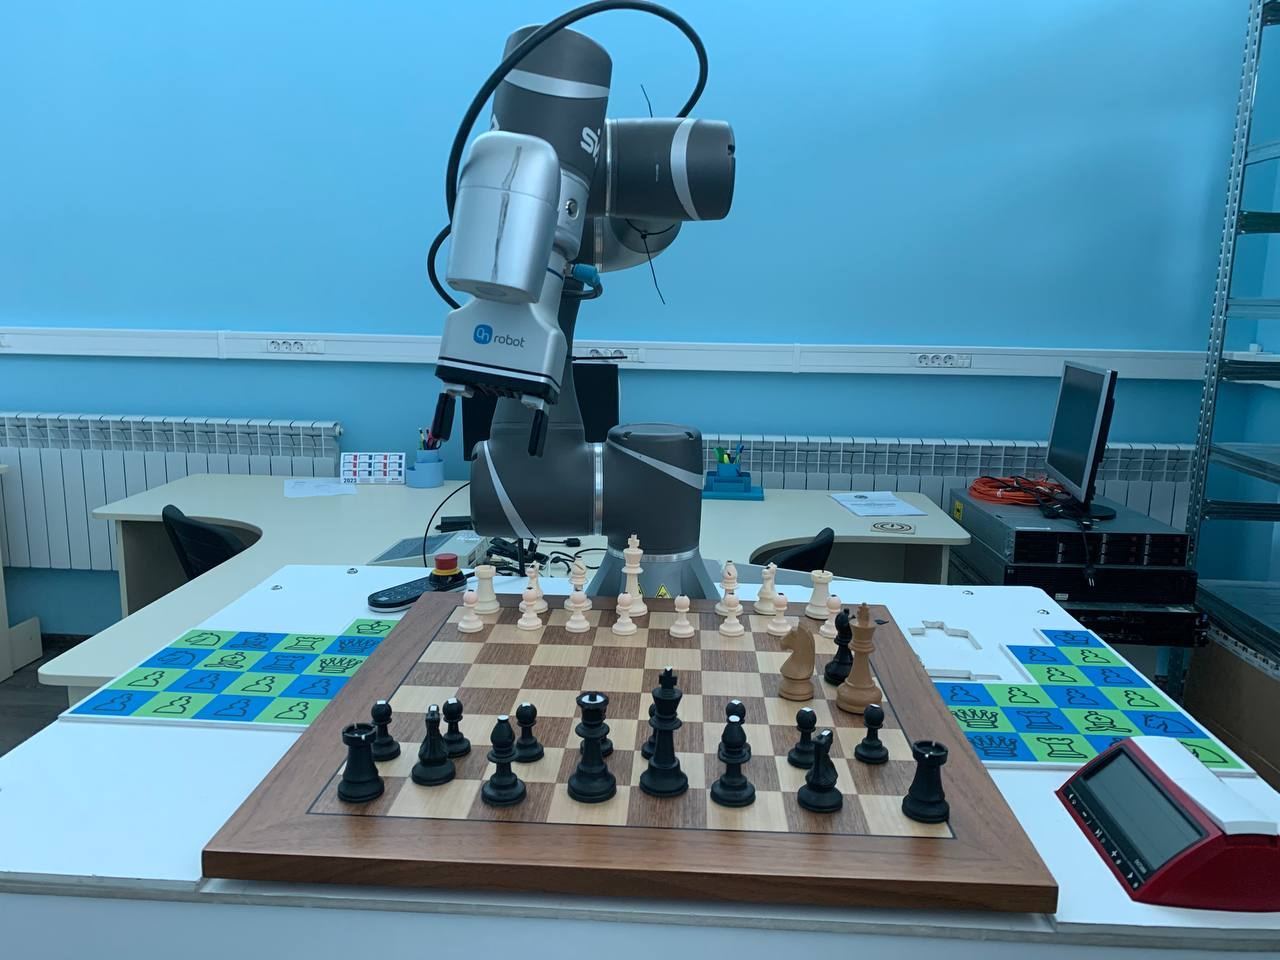
\includegraphics[height=5cm,keepaspectratio]{images/chess.jpg}
		\caption{}
		\label{fig:chess}
	\end{subfigure}
 \hfill
	\begin{subfigure}[b]{0.49\textwidth}
        \centering
		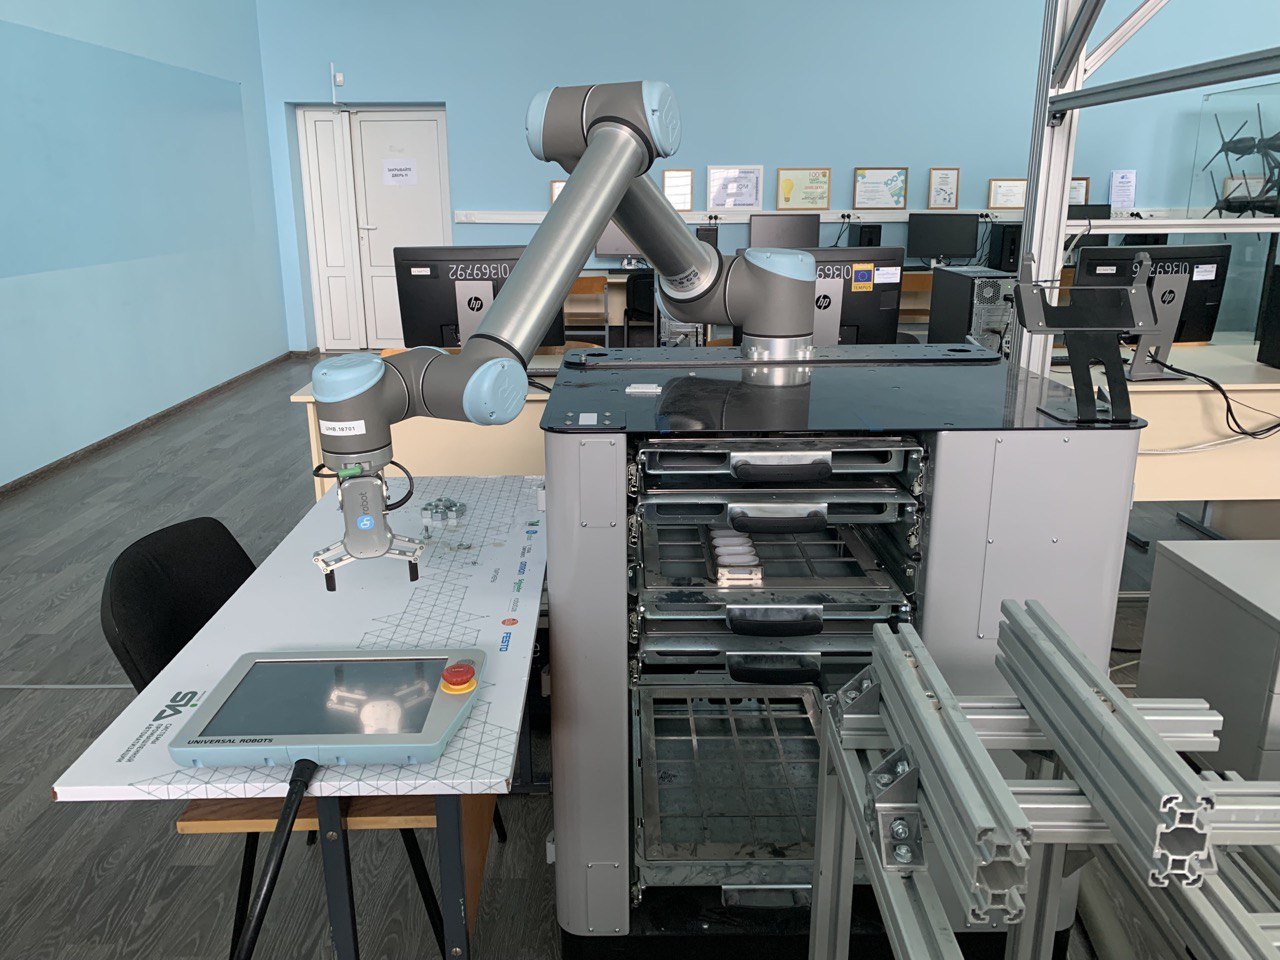
\includegraphics[height=5cm,keepaspectratio]{images/маншир.jpg}
        \caption{}
		\label{fig:маншир}
	\end{subfigure}
 \hspace*{\fill}%
	\begin{subfigure}[b]{0.49\textwidth}
        \centering
		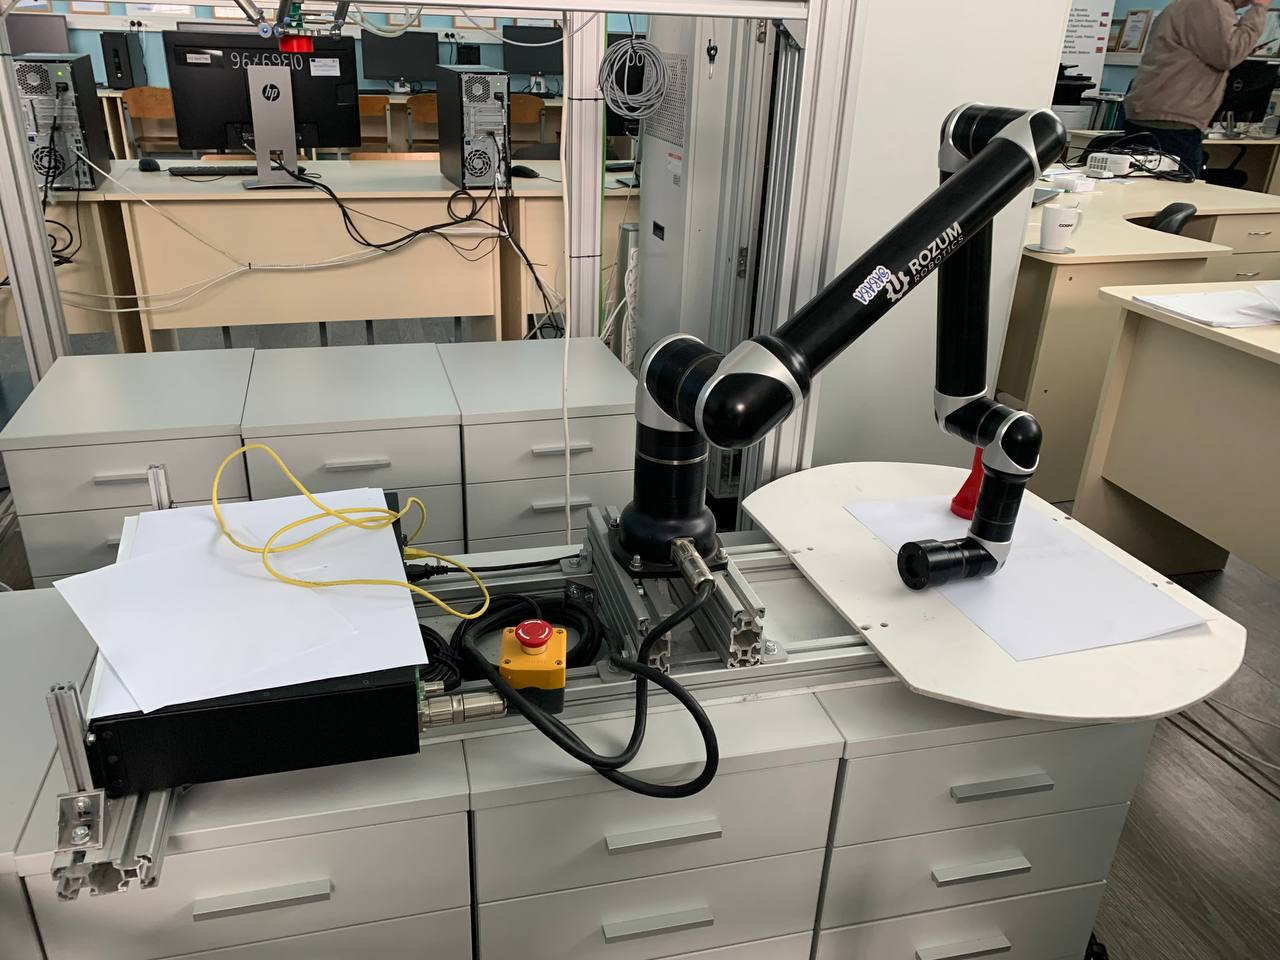
\includegraphics[height=5cm,keepaspectratio]{images/blr.jpg}
		\caption{}
		\label{fig:blr}
	\end{subfigure}
 \hfill
	\begin{subfigure}[b]{0.49\textwidth}
        \centering
		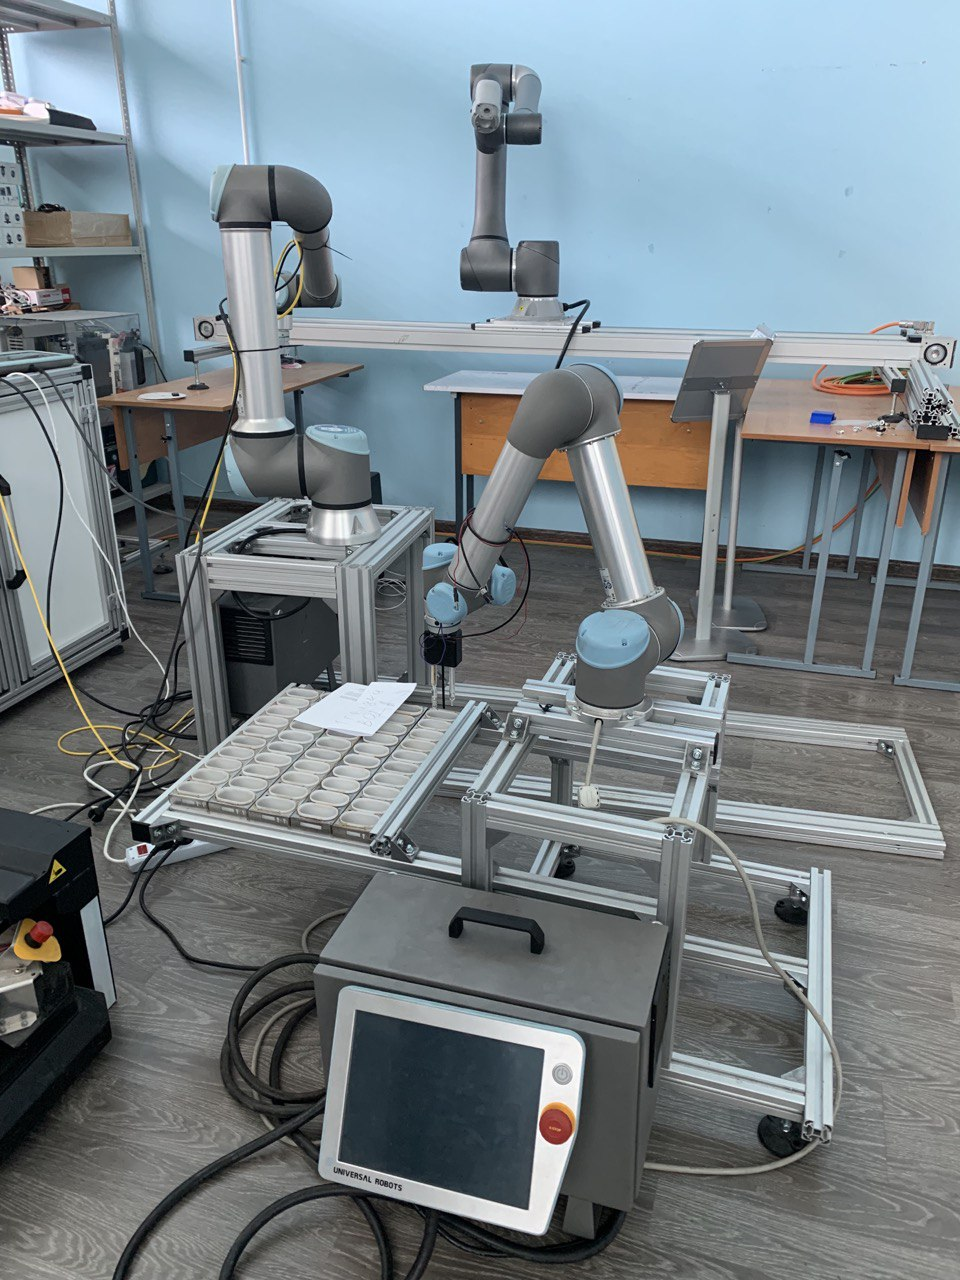
\includegraphics[height=5cm,keepaspectratio]{images/манипулятор.jpg}
        \caption{}
		\label{fig:манипулятор}
	\end{subfigure}

\hspace*{\fill}%
	\caption{Роботы манипуляторы. }
	\label{fig:robot}
 
\end{figure}
 \hfill


 \begin{figure}[ht]
 \centering
		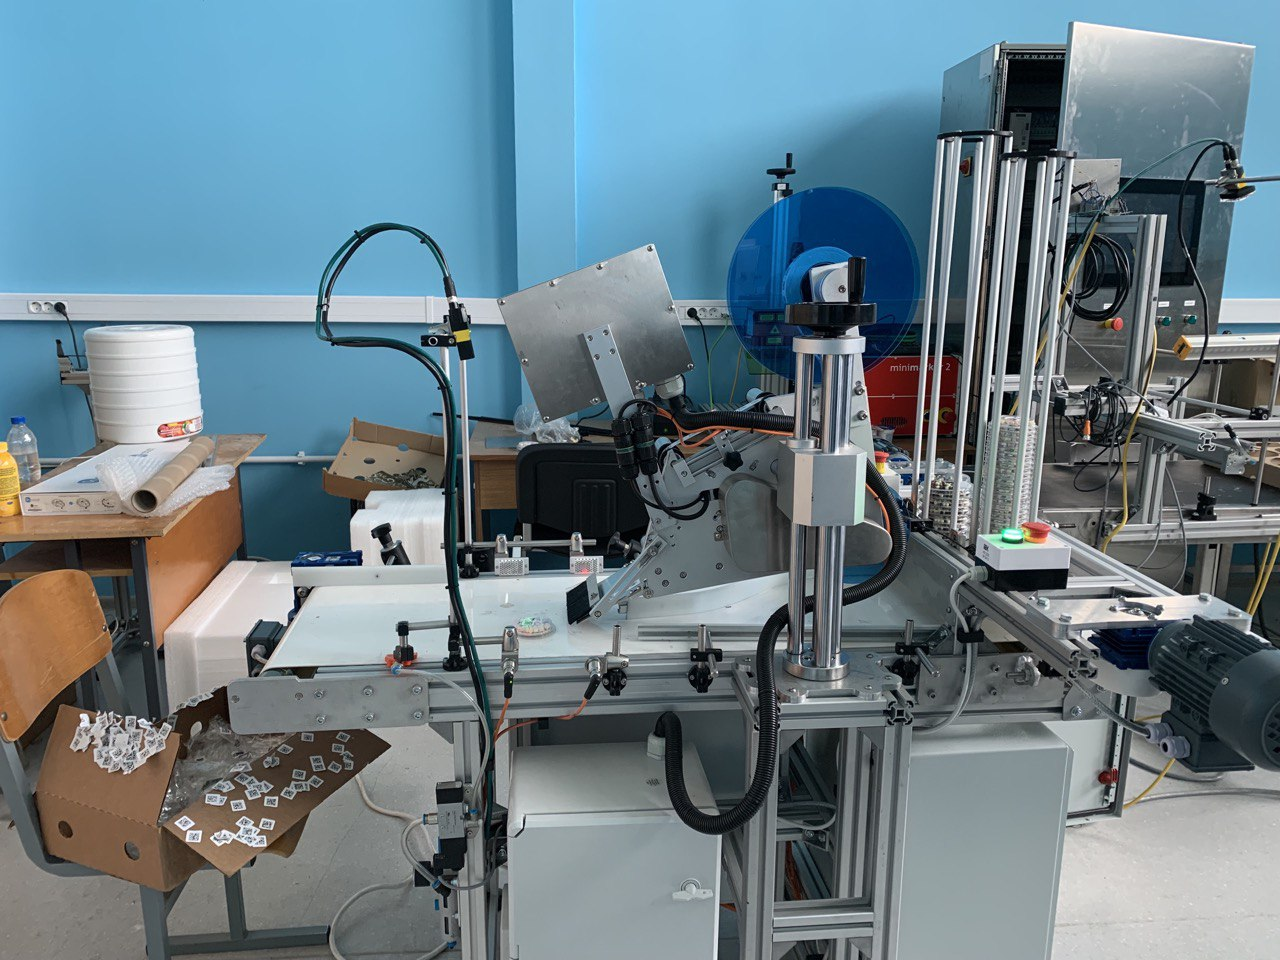
\includegraphics[height =10 cm, keepaspectratio]{images/техзрение.jpg}
		\caption{ Установка для работы с техническим зрением}
		\label{fig:техзрение}
	\end{figure}

\section{ Проделанная работа }

В ходе практики мне довелось заниматься сборкой и запуском проекта на контроллере исходники которого можно найти на GitHub \textcolor{blue}{savushkin-r-d/T1-PLCnext-Demo}, а также обновлением устаревшей документации с помощью Markdown. После запуска данная программа позволяла считывать данные с датчика температуры.
Моим главным заданием на практике было сделать симуляцию датчика температуры при запуске проекта  \textcolor{blue}{savushkin-r-d/ptusa\_main} в режиме эмуляции. То есть программа должна делать вид, что она подключена к контроллеру и считывает данные температуры. Значения температуры должны соответствовать нормальному распределению.

\begin{figure}[ht]
 \centering
		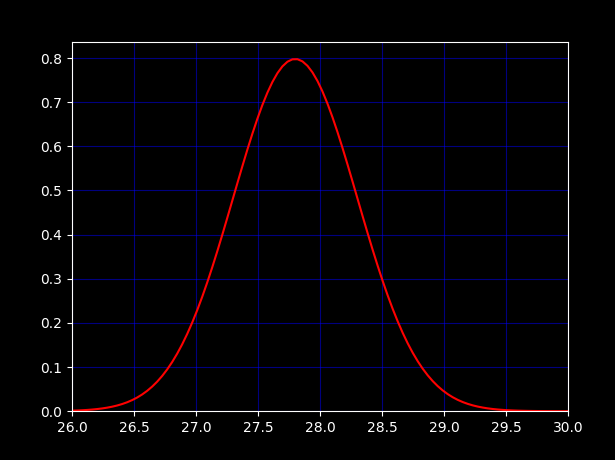
\includegraphics[height =10 cm, keepaspectratio]{images/normal.png}
		\caption{ График функции нормального распределения}
		\label{fig:normal}
	\end{figure}

Для этого мне нужно было разобраться в иерархии классов проекта \textcolor{blue}{ptusa\_main}, изменить функцию получения значений температуры \textcolor{teal}{get\_value()}, написать свой класс \textcolor{teal}{analog\_emulator}, ответственный за возврат значений аналоговых устройств в режиме эмуляции, у которого есть собственный метод \textcolor{teal}{get\_value()}, а затем все это протестировать средствами \textcolor{blue}{googletest} и \textcolor{blue}{github actions}. Все это делолось на языке программирования C++, 11 стандарта. Проект кроссплатформенный и собирается на CMake. Генерацией чисел, которые соответствуют нормальному распределению занималась функция STL \textcolor{teal}{std::normal\_distribution}. Данной функции передаются в качестве параметров мат. ожидание и стандартное отклонение, в программе предусмотрена возможность также в дальнейшем модифицировать эти параметры. Более подробно все изложено в написанном мною {\textcolor{blue}{user\_manual}, Это краткая документация к моему заданию. 

В тестах проверялась правильность инициализации членов класса в конструкторе, работа метода для модификации параметров  в \textcolor{teal}{std::normal\_distribution}.
                                     % Первая глава
\chapter{ ЗАКЛЮЧЕНИЕ    }
\label{ch:concl}

Во время прохождения практики я:
\begin{itemize}
    \item улучшила свои навыки работы с Git
    \item получила опыт работы с реальным проектом
    \item научилась писать документацию к проекту
    \item научилась cобирать и подключать библиотеки к проекту с помощью CMake
    \item изучила материалы и документацию (Matplotlib, Canvas) необходимые для написания дипломной работы
    \item написала публикации по теме дипломной, не без помощи ChatGPT, чтобы получить хотя бы 10 за диплом, т. е. работа с нейросетью
    \item посетила лаборатории «Савушкин продукт» в Политехническом университете
\end{itemize}                                     % Заключение

\end{document}